\newcommand{\Seq}{L0}
\newcommand{\SeqClassParMeth}{L1}
\newcommand{\ParClassSeqMeth}{L2}
\newcommand{\ParClassParMeth}{L3}
\newcommand{\Fork}{F}
\newcommand{\ForkSeq}{\Fork{}\Seq{}}
\newcommand{\ForkParMeth}{\Fork{}\SeqClassParMeth{}}

\section{Parallel Execution of Test Suites}
\label{sec:modes}

\begin{figure}[t!]
  \centering
  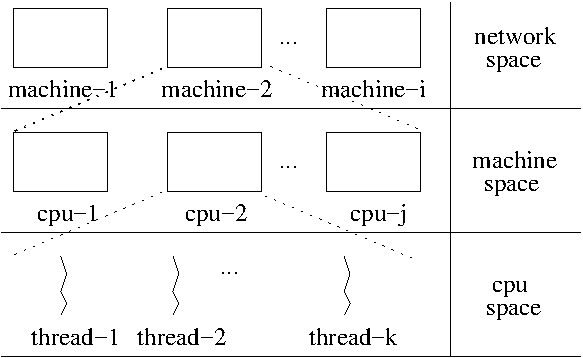
\includegraphics[width=0.35\textwidth]{figs/parallel-levels.pdf}
  \vspace{-1ex}
  \caption{\label{fig:levels}Levels of parallelism.}
\end{figure}

%\Mar{add a sentence to introduce this section at a higher abstraction
%  level.}

This section provides some background on parallel test execution.

Parallelism in test execution can be obtained at different levels.
Figure~\ref{fig:levels} illustrates relevant levels.  The highest
level indicates parallelism that can be obtained through different
machines on the network.  For instance, using virtual machines from a
cloud service to perform a distributed execution.  The machine space
sits under the ``network space'' and provides a \emph{lower-level}
parallelism.  In this case, computation can be offloaded at different
CPUs within a machine and at different threads within each CPU.  Note
that all these levels are complementary:  low-level parallelization
schemes could leverage the computing power of server nodes in addition
to the aggregate processing power of the farm.

%% Lower-level parallelism fits
%% particularly well smaller organizations (/projects) with relatively
%% high testing costs but lower budgets.

This paper focuses at low-level parallelism (\ie, machine and CPU
space), which can be enabled through build systems and testing
frameworks.  Given the proliferation of multi-core machines it is not
surprising that testing frameworks provide today support for parallel
test execution (e.g., JUnit~\cite{junit-org}, TestNG~\cite{testng},
and NUnit~\cite{nunit}).  In the following we elaborate relevant
features of and testing frameworks build systems.  We focused on Java,
Maven, and JUnit but the discussion can be generalized to other
language and tools.

\Comment{
    Unfortunately, these solutions can't be used out-of-the-box:
    unrestricted parallel execution of tests can produce
    non-deterministic results as developers typically do not provision
    protection to concurrent accesses originated from arbitrary program
    points (\ie{}, tests).  We refer to this problem as Parallel
    Execution Flakiness (\pef{}).

    %% These solutions enable the
    %% use of commodity hardware to maximize CPU usage\footnote{In the case
    %%   of the Java language, for example, it is possible to explore
    %%   parallelism across and within JVMs.}.  

    To illustrate the importance of parallel test execution and
    the problem of \pef{} let's consider the case of the ``core'' module
    from the Apache Camel project~\cite{apache-camel-web}.  This module
    contains 5,679 test cases, declared in 2,356 test classes.  We ran
    those tests in a machine with 16GB of memory and 8 virtual CPUs (4
    cores with 2 native threads each).  Sequential test execution takes
    24m50s to run this test set.  Execution of the same test set takes
    2m28s when we configured parallel execution to fork a JVM per CPU and
    execute test classes, uniquely allocated to that JVM, sequentially but
    running test methods from each class in separate threads.  Note that
    this is an order of magnitude speedup (10.07x)\Fix{Need to understand
    why this is 10x as opposed to something closer to 7x - I didn't get
    your concern here}.  Unfortunately, due to \pef{}, $\sim$2\% (114 of
    5,679) of the tests fail when executed in parallel.  It is important
    to notice that the ratio of failures varies with the project as it
    depends on factors such as length of test cases and amount of shared
    state across tests.

    \pef{} is an important obstacle to enable parallel test execution.
    Conceptually, higher parallelization can result in higher chances of
    concurrency-related problems.  It is important to execute tests
    efficiently without sacrificing reliability
    \Fix{gap between pars?? What gap?}
}

%%Build systems delegate functionalities to the testing framework they
%%use~\cite{maven-surefire-plugin}.  Figure~\ref{fig:surefire}
%%illustrates how to configure Maven for mode
%%\ParClassSeqMeth{}~--~classes sequentially (default) and test methods
%%in parallel. Although this configuration is defined in the build file
%%(\eg, \emph{pom.xml} on Maven), these settings are forwarded to the
%%underlying testing framework (in this case, JUnit).

%% \Jbc{I have to understand better how Surefire executes tests. I'm
%% afraid it has its own wrapper classes and reuse JUnit core
%% functionalities. I'm saying this because JUnit does not offer a finer
%% control over thread numbers while this configuration is possible with
%% Surefire} For example,

%\Fix{we
%  need to know how Maven allocates test classes to JVMs}

\subsection{Testing Frameworks}
\label{sec:frameworks}

The list below shortly describes the choices to control parallelism
within a Java virtual machine (JVM).

\begin{itemize}
\item
    \textbf{Sequential (\Seq).}~This configuration corresponds to the
        default behaviour in a test execution. No parallelism is
        involved.
\item
    \textbf{Sequential classes; parallel methods
        (\SeqClassParMeth).}~When running a test class, the testing
        framework executes methods on multiple threads. Each class
        runs sequentially.
\item
    \textbf{Parallel classes; sequential methods
        (\ParClassSeqMeth{}).}~The testing framework runs test classes
        on multiple threads and methods run sequentially within each
        thread.
\item
    \textbf{Parallel classes; Parallel methods
        (\ParClassParMeth).}~This configuration corresponds
        conceptually to the union of \ParClassSeqMeth{} and
        \SeqClassParMeth{}: the testing framework runs test methods
        from several classes on multiple threads.
\end{itemize}

Typically, testing frameworks executes tests in sequence by default
(\Seq{}) and may allow the developer to use an ordering criteria (\eg,
test name).  For the \SeqClassParMeth{} setting, \Fix{elaborate...}.
For the \ParClassSeqMeth{} setting, \Fix{elaborate...}. Finally, the
\ParClassParMeth{} setting \Fix{...elaborate...}.

\subsection{Build Systems}
\label{sec:builder}

The list below shortly describes the choices to control parallelism
through build systems:

\begin{itemize}
\item
    \textbf{Forked classes; sequential methods (\ForkSeq).}~This
        configuration corresponds to the parallel execution of test
        classes on different JVMs and test methods run sequentially
        within each JVM.
\item
    \textbf{Forked classes; parallel methods (\ForkParMeth).}~This
        configuration corresponds to the parallel execution of test
        classes on different JVMs and test methods run on multiple
        threads within each JVM.
\end{itemize}

Several build systems support the execution of test classes in forked
processes running a JVM. In the \ForkSeq{} configuration, each spawned
process runs a different test class at time and the builder merges the
results from each execution. In the \ForkParMeth{} configuration, the
build system forwards settings to the underlying testing framework to
enable parallel execution within each process in addition to running
test classes on different processes.  However, some configurations
(\eg, \ParClassSeqMeth) may not take effect since only one test class
can run in a forked process at time.  To the best of our knowledge, we
are unaware of any build system capable of running multiple classes at
time within a forked process.  \Comment{In addition, the builder can
reuse these processes to execute the next test classes in the queue
according to the developer's preference. For instance, one might want
the builder to spawn a new process for each test class to ensure
maximum isolation. Notice that to exploit parallelism at build system
level, the number of forked processes must be proportional to the
number of available CPUs, otherwise, the high frequency of
context-switching and processes competing for a CPU may degrade the
execution performance  \Jbc{$\leftarrow$ I'm not sure if we should
keep this. We can remove it if necessary}.}

%% In this paper, we use the prefix ``\Fork{}'' to indicate that a given
%% testing configuration has the feature of spawning JVMs to run test
%% classes enabled.

\subsubsection*{Illustration}~\Fix{elaborate the following example to
conclude this section}

\begin{figure}[h!]
\centering
\scriptsize
\lstset{
    escapeinside={@}{@},
    numbers=left,xleftmargin=1em,frame=single,framexleftmargin=0.5em,
    basicstyle=\ttfamily\scriptsize, boxpos=c, numberstyle=\tiny,
    morekeywords={parallel, threadCount, perCoreThreadCount,
    forkCount, reuseFork},
    deletekeywords={true}
}
\begin{lstlisting}
<plugin>
    <groupId>org.apache.maven.plugins</groupId>
    <artifactId>maven-surefire-plugin</artifactId>
    <configuration>
        <forkCount>1C</forkCount>
        <parallel>methods</parallel>
        <threadCount>5</threadCount>
    </configuration>
</plugin>
\end{lstlisting}
    \caption{\label{fig:surefire} Maven with a \ForkParMeth{}
    configuration. Maven forks one JVM per core (\CodeIn{forkCount}
    parameter) and \Jbc{check this $\rightarrow$} uses five threads
    (\CodeIn{threadCount} parameter) to run methods (\CodeIn{parallel}
    parameter) within each JVM.}
    
%%    test methods run in parallel (\CodeIn{parallel}
%%    parameter) using two threads (\CodeIn{threadCount} parameter) per
%%    available core (flag \CodeIn{perCoreThreadCount}).}
\end{figure}

%% \Fix{-----}
%% In JUnit, \emph{ParallelComputer} provides support to parallel
%% execution: it instantiates a test runner with an
%% \emph{ExecutorService} from the Java Concurrent API. Each test method
%% is executed in a separated thread as the thread pool creates new
%% threads on-demand and reuse them if any thread is available.
%% \Comment{http://junit.org/junit4/javadoc/latest/src-html/org/junit/experimental/ParallelComputer.html#line.14}

%% As in \ParClassSeqMeth, the test runner has a cached thread poll but
%% instead of executing test methods from a single test class, the test
%% suite runner executes classes in separated threads and methods
%% sequentially within each thread.

%% \Jbc{I need to confirm this but AFAIK this is how it happens} As in
%% \SeqClassParMeth, classes execute on separated threads but test
%% methods are also executed in parallel. More precisely, there is a
%% thread pool to execute classes in separated threads (\ie, like in
%% \ParClassSeqMeth) and, within each class runner, there is an
%% \emph{ExecutorService} to run test methods in parallel (\ie, like in
%% \SeqClassParMeth).

%% \Fix{-----}

